\documentclass{beamer}
\usetheme{Madrid}
\usepackage{graphicx}
\usepackage{subcaption}
\usepackage{booktabs}

\title[Factory Electric Consumption Prediction]{Factory Electric Consumption Prediction}
\subtitle{A Regression-Based Forecasting Approach}
\author{Irene Burri}
\date{April 15, 2025}

\begin{document}

% Title Slide
\begin{frame}
  \titlepage
\end{frame}

% Project Objective
\begin{frame}{Project Objective}
  \begin{itemize}
    \item Develop a regression model to predict future electric consumption in a factory.
    \item Optimize energy usage, reduce costs, and support sustainability.
    \item Evaluation metric: \textbf{Root Mean Squared Error (RMSE)}.
  \end{itemize}
\end{frame}

% Motivation
\begin{frame}{Motivation}
  \begin{itemize}
    \item Rising energy costs and sustainability goals.
    \item Accurate forecasts enable better planning and optimization.
    \item Opportunity to identify seasonal trends and usage anomalies.
  \end{itemize}
\end{frame}

% Dataset Overview
\begin{frame}{Dataset Overview}
  \begin{itemize}
    \item \textbf{Training data:} 13,872 records
    \item \textbf{Test data:} 2,160 records
    \item \textbf{Target:} \textbf{Electric\_Consumption}
    \item Provided by Kaggle: \url{https://www.kaggle.com/competitions/prediction-of-factory-electric-consumption/}
  \end{itemize}
\end{frame}

% Tools and Libraries
\begin{frame}{Tools and Libraries}
  \begin{itemize}
    \item Python, Pandas, NumPy
    \item Scikit-learn, XGBoost
    \item Matplotlib, Seaborn
    \item GridSearchCV for hyperparameter tuning
  \end{itemize}
\end{frame}

% Data Preprocessing
\begin{frame}{Data Processing Steps}
\begin{itemize}
    \item Date Formatting and Feature Extraction of time-based features (Hour, Day, Month, DayOfWeek)
    \item Outlier Detection and Clipping
    \item Handling Missing Values
    \item Encoding Categorical Features (Cyclical Encoding)
\end{itemize}
\begin{figure}
    \centering
    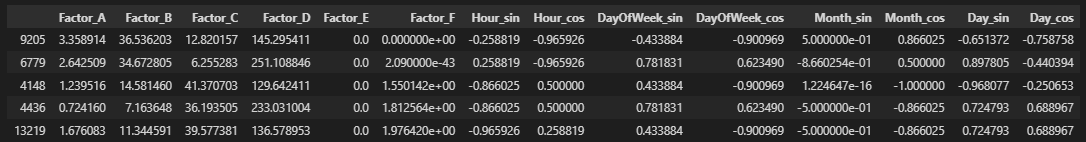
\includegraphics[width=0.9\linewidth]{images/Xtrain_head.png}
    \caption{X\_train head after Data preprocessing}
    \label{fig:enter-label}
\end{figure}
\end{frame}

%Exploratory Data Analysis
\begin{frame}{Exploratory Data Analysis}
\begin{itemize}
    \item Boxplots and Distribution plots used for outlier analysis
    \item Correlation analysis to identify key features
    \item Visualizations of electric consumption trends
\end{itemize}
\begin{figure}
    \centering
    \begin{subfigure}[t]{0.48\textwidth}
        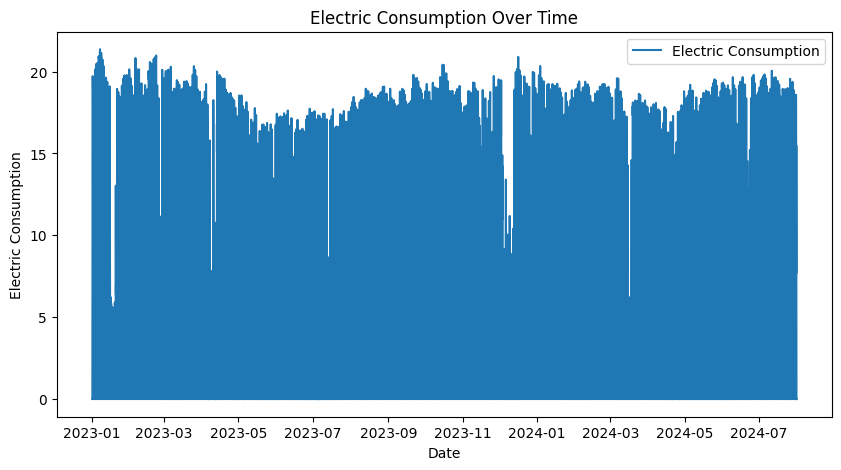
\includegraphics[width=\linewidth]{images/EC_Time.png}
        \caption{Electric\_Consumption over Time}
    \end{subfigure}
    \hfill
    \begin{subfigure}[t]{0.48\textwidth}
        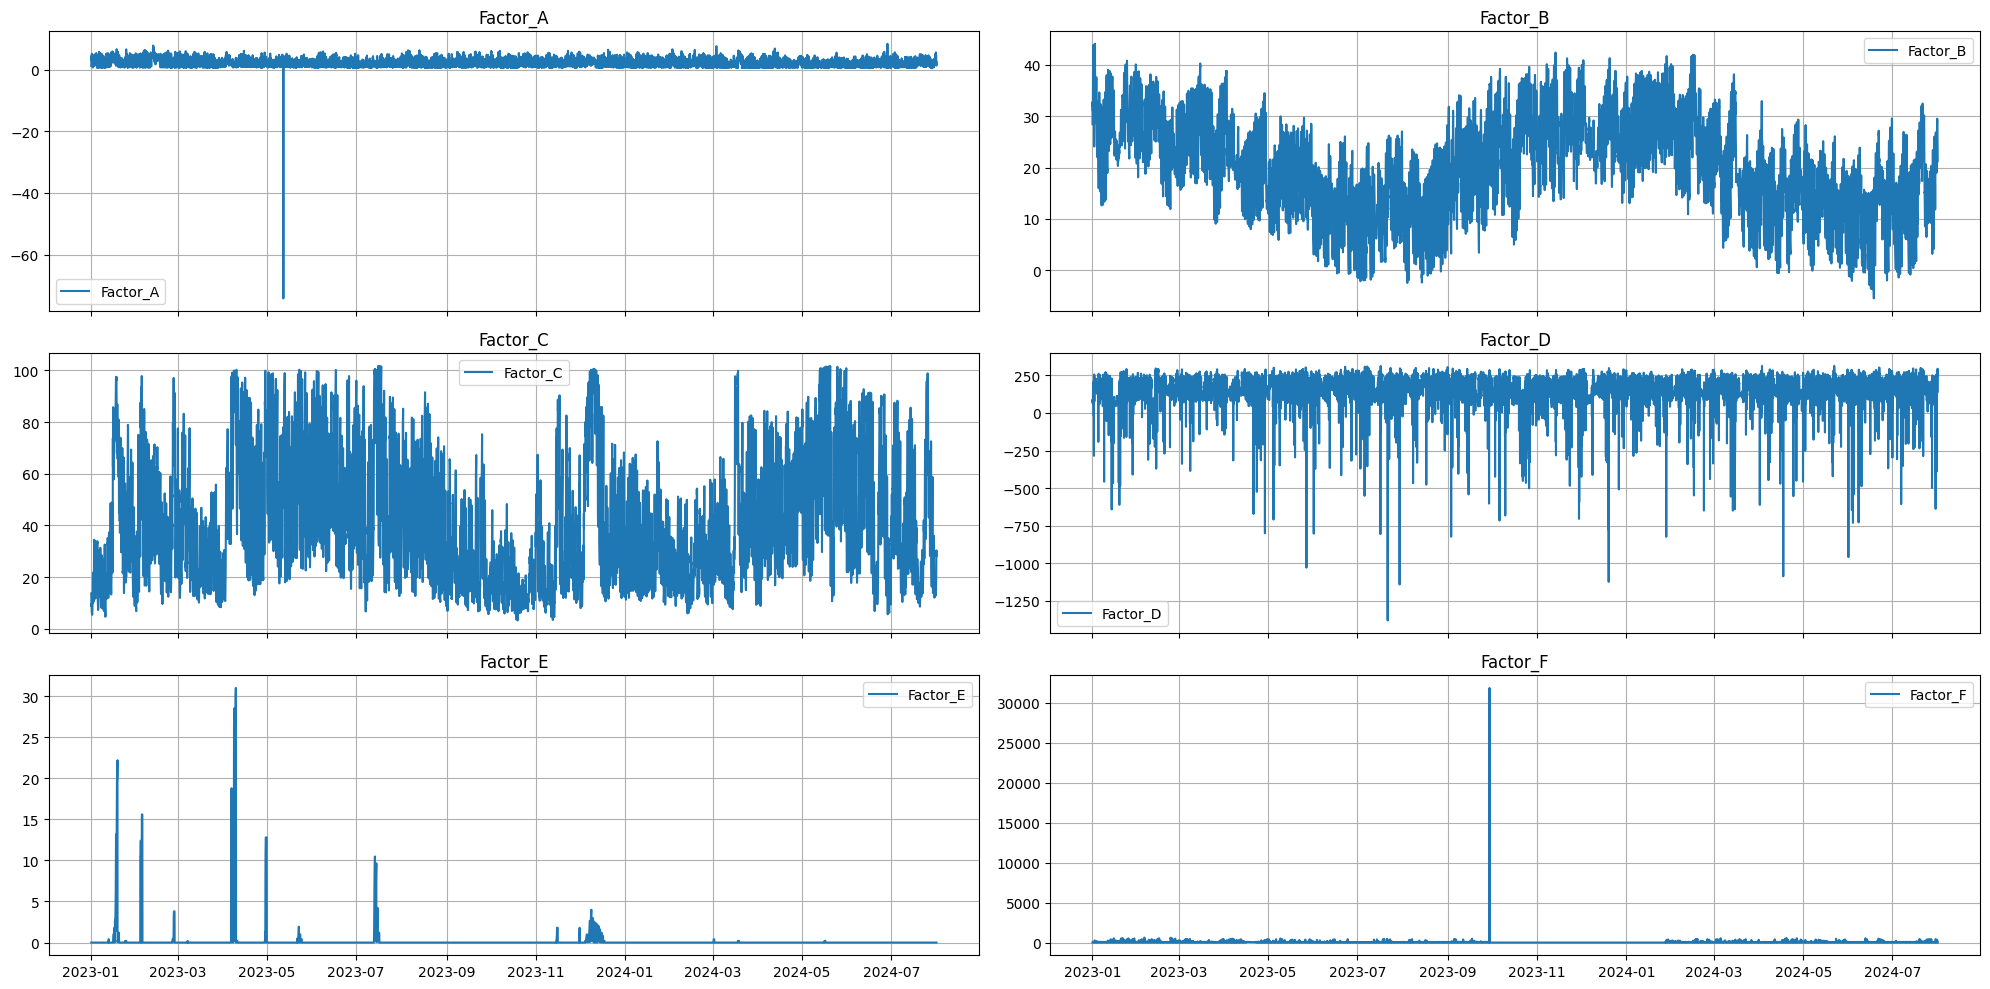
\includegraphics[width=\linewidth]{images/Factors_Time.png}
        \caption{Factors trend over Time}
    \end{subfigure}
\end{figure}
% \begin{figure}
%     \centering
%     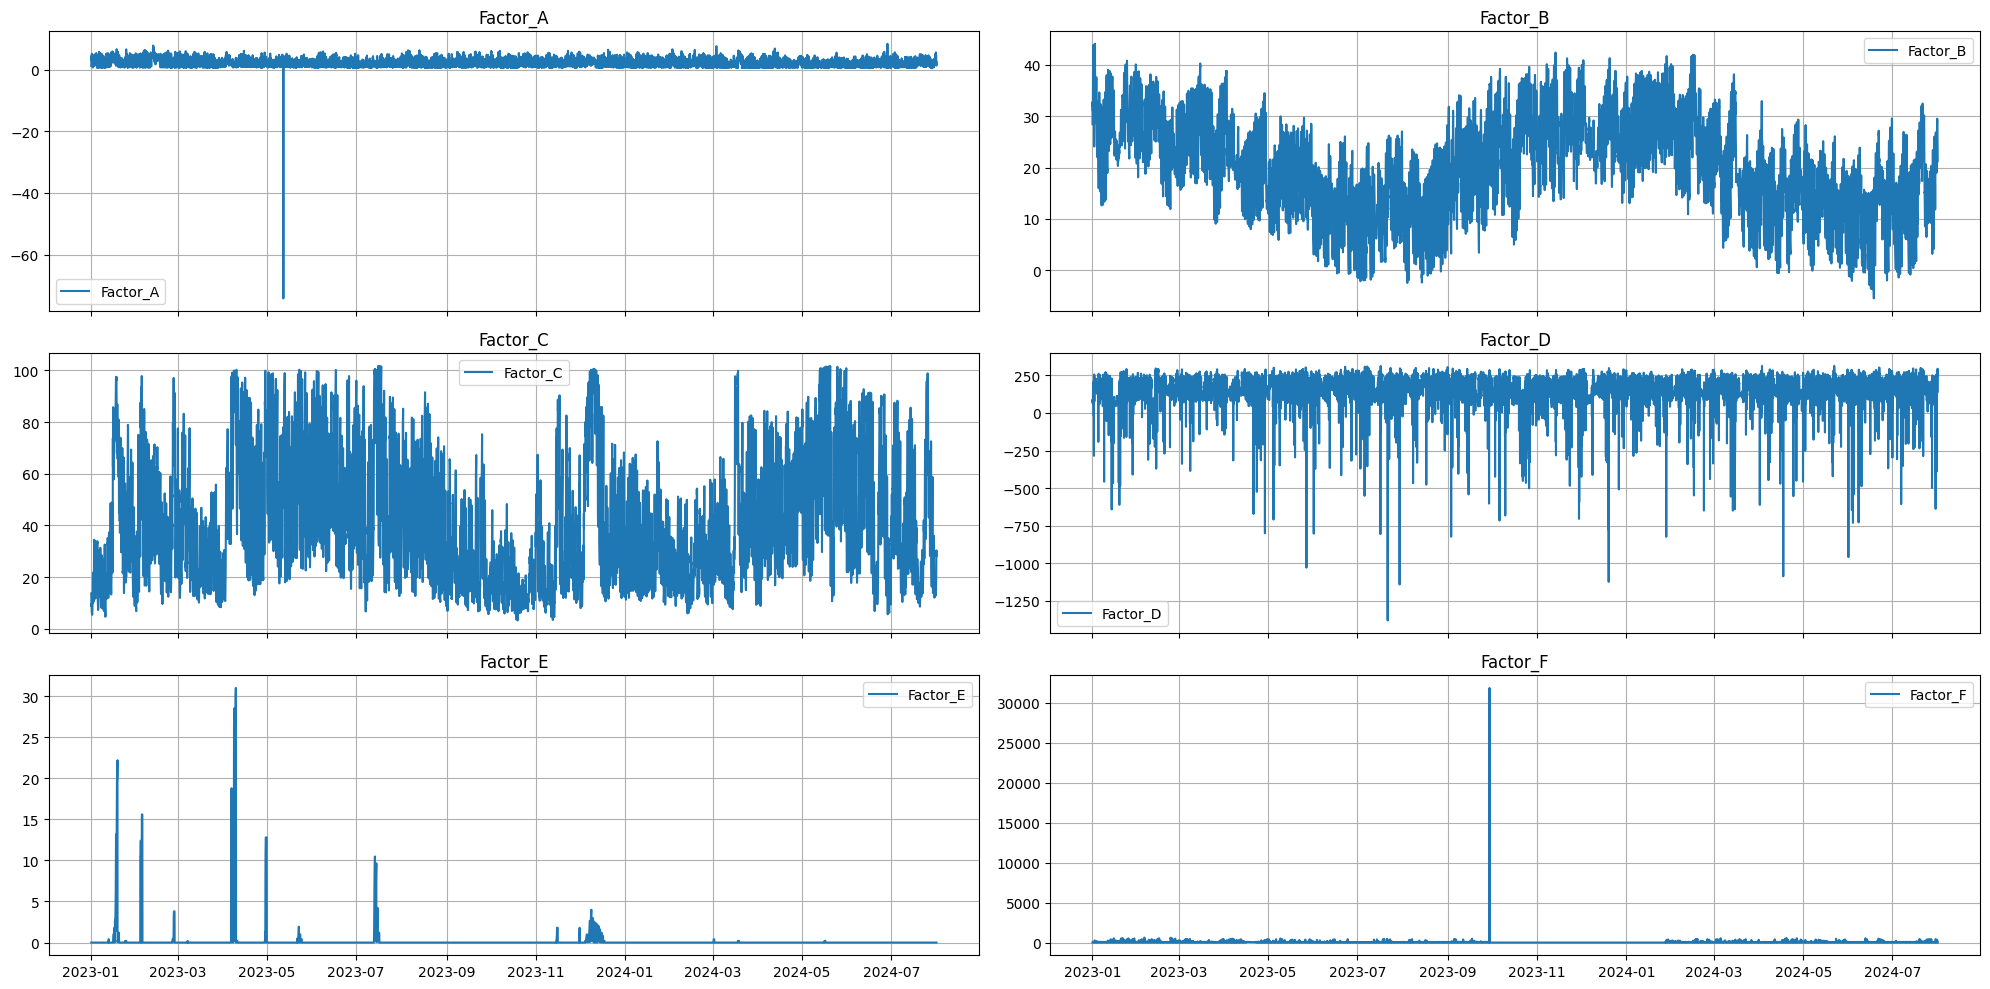
\includegraphics[width=0.4\linewidth]{images/Factors_Time.png}
%     \caption{Electric consumption trend over time}
%     \label{fig:enter-label}
% \end{figure}
\end{frame}

% \begin{center}
% \begin{minipage}{0.48\textwidth}
%     \centering
%     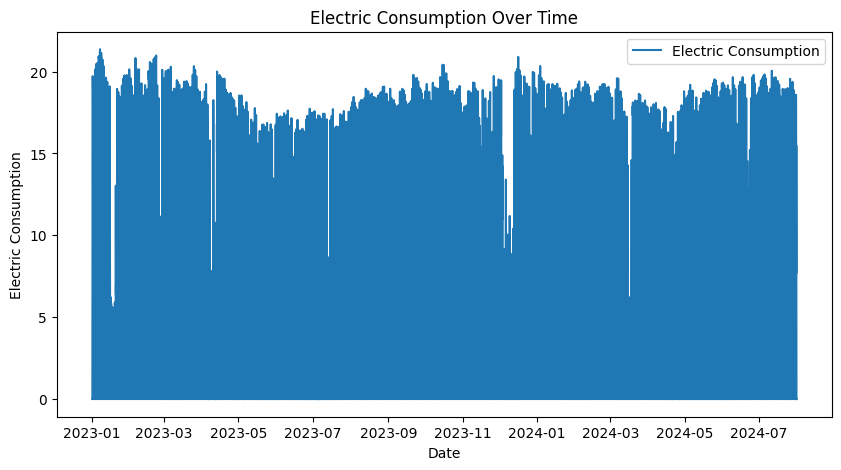
\includegraphics[width=\linewidth]{images/EC_Time.png}
%     \caption*{Feature Importance - XGBoost}
% \end{minipage}
% \hfill
% \begin{minipage}{0.48\textwidth}
%     \centering
%     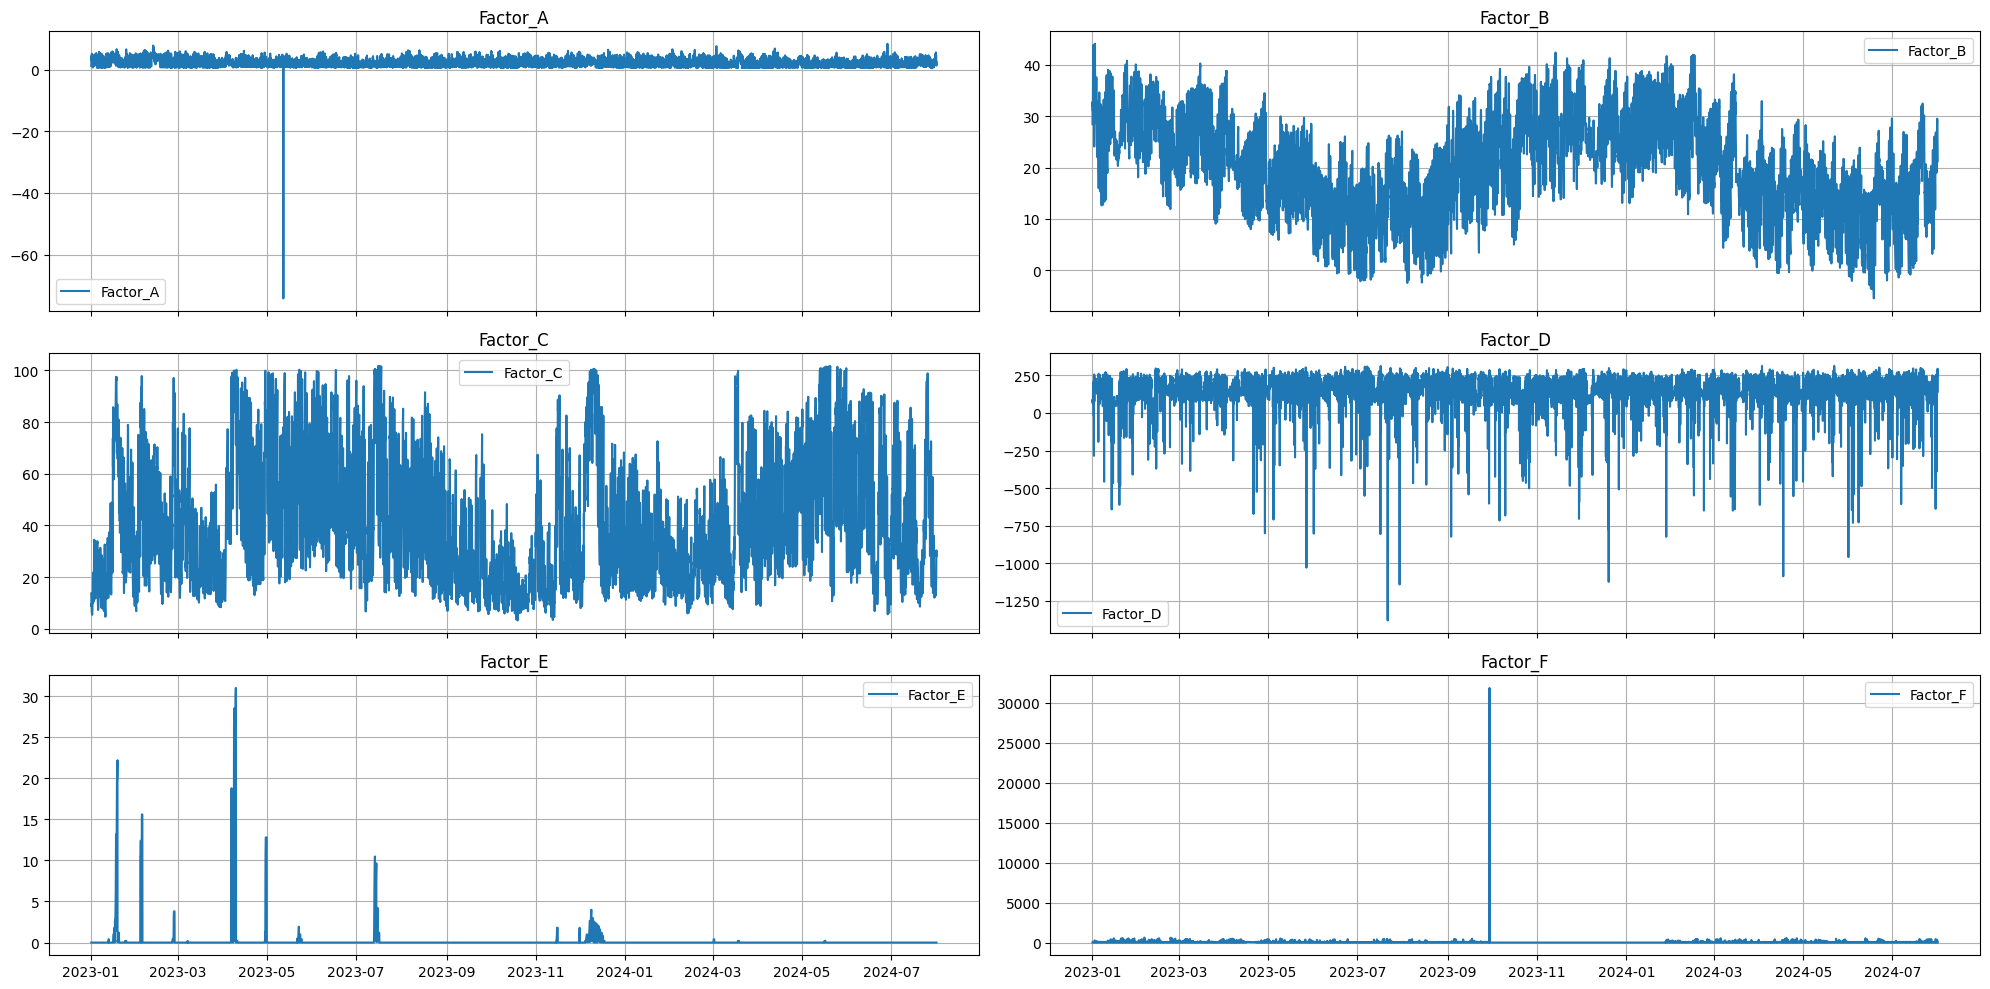
\includegraphics[width=\linewidth]{images/Factors_Time.png}
%     \caption*{Feature Importance - Random Forest}
% \end{minipage}
% \end{center}

% Models Training and Evaluation
\begin{frame}{Models Used}
\begin{itemize}
    \item Linear Regression
    \item Polynomial Regression (with Hyperparameters Tuning)
    \item Random Forest Regressor (with Hyperparameters Tuning)
    \item XGBoost Regressor (with Hyperparameters Tuning)
\end{itemize}
\end{frame}

\begin{frame}{Model Evaluation Criteria}
\begin{itemize}
    \item Cross-Validation RMSE
    \item Validation RMSE
    \item Hyperparameter tuning using GridSearchCV
    \item Feature Importance Analysis
    \item Post-processing to avoid negative predictions
\end{itemize}
\end{frame}
    
% Linear Regression
\begin{frame}{Model: Linear Regression}
  \begin{itemize}
    \item Simple baseline model
    \item Fast to train but limited in performance
    \item \textbf{Validation RMSE:} 3.19
  \end{itemize}
\begin{figure}
\vfill
    \centering
    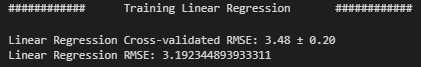
\includegraphics[width=0.6\linewidth]{images/lr.png}
    \caption{Training Linear Regressor}
    \label{fig:enter-label}
\end{figure}
\end{frame}

% Polynomial Regression
\begin{frame}{Model: Polynomial Regression}
  \begin{itemize}
    \item Captures non-linear relationships
    \item Tuned degree and bias 
        \begin{itemize}
            \item degree = 2,
            \item include\_bias = True
        \end{itemize}  
    \item \textbf{Validation RMSE:} 2.24
  \end{itemize}
  \begin{figure}
\vfill
    \centering
    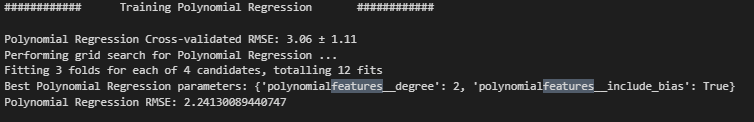
\includegraphics[width=0.6\linewidth]{images/pr.png}
    \caption{Training Polynomial Regressor}
    \label{fig:enter-label}
\end{figure}
\end{frame}

% Random Forest
\begin{frame}{Model: Random Forest Regressor}
  \begin{itemize}
    \item Ensemble of decision trees
    \item Tuned hyperparameters via GridSearchCV:
        \begin{itemize}
            \item max\_depth = None
            \item min\_sample = 2
            \item n\_estimators = 200
        \end{itemize}  
    \item \textbf{Validation RMSE:} 1.67
  \end{itemize}
  \begin{figure}
\vfill
    \centering
    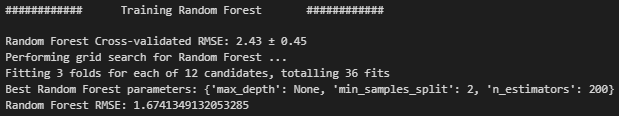
\includegraphics[width=0.6\linewidth]{images/rf.png}
    \caption{Training Random Forest Regressor}
    \label{fig:enter-label}
\end{figure}
\end{frame}

% XGBoost
\begin{frame}{Model: XGBoost Regressor}
  \begin{itemize}
    \item Gradient Boosting-based model
    \item Best hyperparameters:
    \begin{itemize}
        \item learning\_rate = 0.05, max\_depth = 6
        \item n\_estimators = 1000, subsample = 0.8
    \end{itemize}
    \item \textbf{Validation RMSE:} \textbf{1.49} (Best)
  \end{itemize}
  \begin{figure}
\vfill
    \centering
    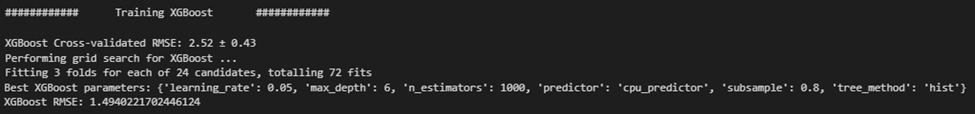
\includegraphics[width=0.6\linewidth]{images/xgboost.png}
    \caption{Training XGBoost Regressor}
    \label{fig:enter-label}
\end{figure}
\end{frame}

% Post-processing
\begin{frame}{Post-processing}
  \begin{itemize}
    \item Ensured no negative consumption values.
    \item Applied post-processing to clip predictions to zero minimum.
  \end{itemize}
\end{frame}

% Performance Comparison
\begin{frame}{Performance Comparison}
\small
    \begin{tabular}{lccc}
        \toprule
        \textbf{Model} & \textbf{CV RMSE ± std} & \textbf{RMSE} & \textbf{Best Params} \\
        \midrule
        Linear Reg. & 3.48 ± 0.20 & 3.19 & Default \\
        &&&\\
        Poly. Reg. & 3.06 ± 1.11 & 2.24 & deg=2, include\_bias=True \\
        &&&\\
        Random Forest & 2.43 ± 0.45 & 1.67 & est=200, depth=None, \\ &&&min\_sample\_split=2 \\
        &&&\\
        \textbf{XGBoost} & 2.52 ± 0.43 & \textbf{1.49} & lr=0.05, depth=6, est=1000,\\ &&&subsample=0.8\\
        \bottomrule
    \end{tabular}
\end{frame}


% Model Comparison
\begin{frame}{Model Comparison}
  \begin{itemize}
    \item XGBoost achieved the best performance but took more time.
    \item Random Forest also performed well with low variance.
    \item Polynomial Regression improved over linear baseline.
  \end{itemize}
\end{frame}

\begin{frame}{Feature Importance}
\begin{itemize}
    \item XGBoost and Random Forest revealed most influential features.
    \item Attempts to remove less important features degraded model performance.
    \item All available engineered features retained for final model.
\end{itemize}
  \begin{figure}
\vfill
    \centering
    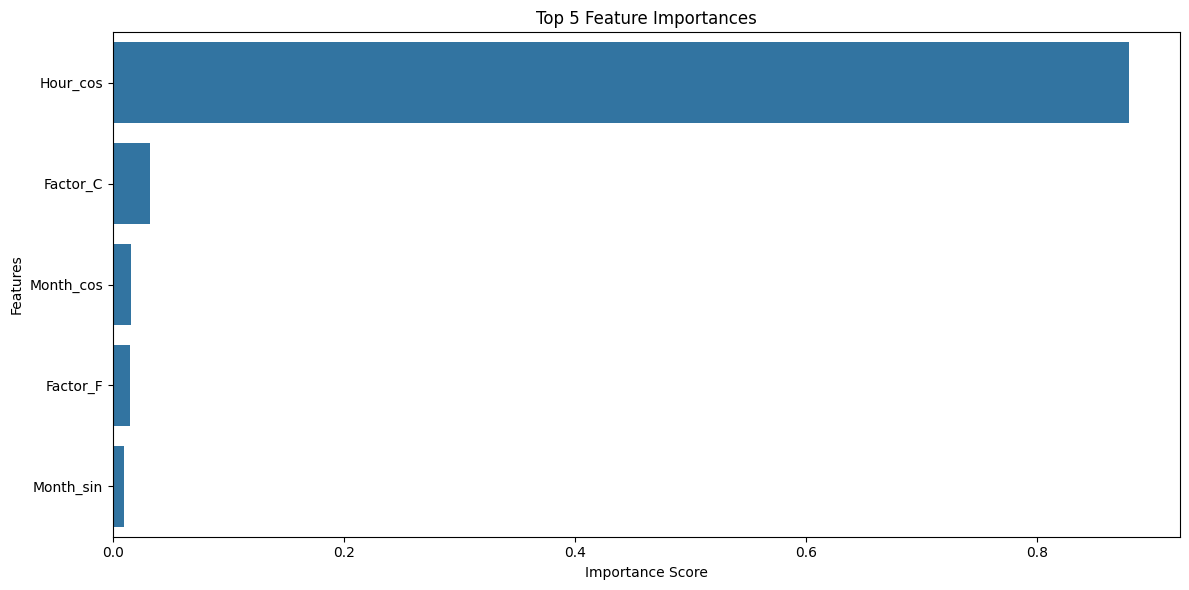
\includegraphics[width=0.6\linewidth]{images/fi_xgb.png}
    \caption{Top 5 Feature Importances}
    \label{fig:enter-label}
\end{figure}
\end{frame}

\begin{frame}{Final Model}
\begin{itemize}
    \item \textbf{Best model: XGBoost Regressor}
    \item Final RMSE on validation set: \textbf{1.49}
    \item Cleaned and well-engineered features contribute to high performance.
    \item Further improvements may be possible with deep learning.
\end{itemize}
\end{frame}

% Conclusion
\begin{frame}{Conclusion}
  \begin{itemize}
    \item Successfully predicted factory electricity usage using regression models.
    \item XGBoost yielded best performance (RMSE = 1.49).
    \item Insights can support sustainable and cost-effective energy management.
  \end{itemize}
    \begin{figure}
\vfill
    \centering
    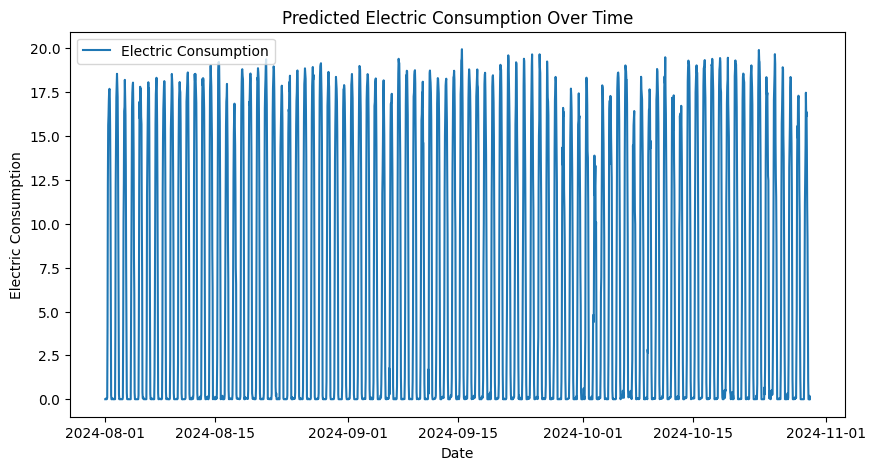
\includegraphics[width=0.5\linewidth]{images/predictedEC.png}
    \caption{Predicted Electric Consumption over Time}
    \label{fig:enter-label}
\end{figure}
\end{frame}

% References
\begin{frame}{References}
  \begin{itemize}
    \item Kaggle Competition: \url{https://www.kaggle.com/competitions/prediction-of-factory-electric-consumption/}
    \item Scikit-learn, XGBoost Documentation
    \item GitHub project repository: \url{https://github.com/ireneburri/Burri-PredictionOfFactoryElectricConsumption.git}
  \end{itemize}
\end{frame}

\end{document}




